\documentclass[letterpaper, 10pt]{article}

\usepackage{amsmath}
\usepackage{float} 
\usepackage{graphicx}
\usepackage{gensymb}

\usepackage[margin=1in]{geometry}

\title{Radio Background Research Notes}
\author{Nitika Yadlapalli}
\date{}


\begin{document}
\maketitle

\section{Sky Brightness Model for a Disk+Halo and Extragalactic Sources}

\subsection{Contribution from Disk}
Given a pair of galactic coordinates, we need to determine the line of sight through the disk. This, combined with the emissivity of the disk, will allow us to know flux density contributed by the disk.

\begin{figure}[h]
\begin{center}
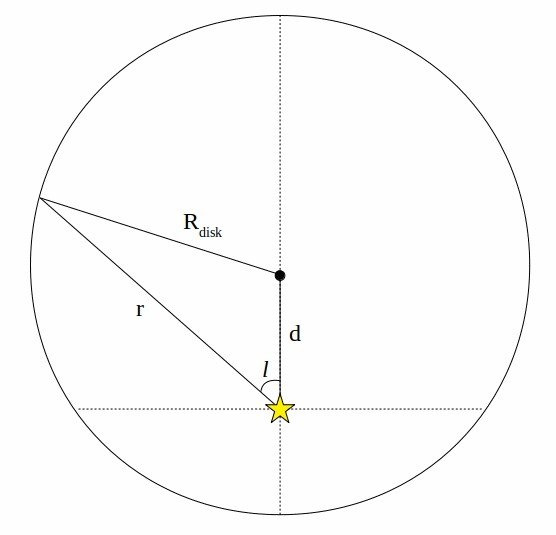
\includegraphics[width=0.39\textwidth]{disk_face.jpg}
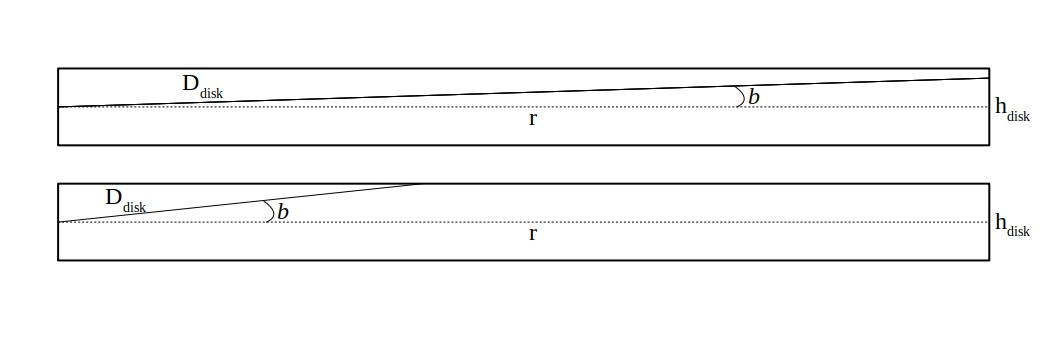
\includegraphics[width=0.59\textwidth]{disk_edge.jpg}
\caption{Two views of disk, face on and edge on, illustrating how line of sight through disk is calculated}
\label{disk}
\end{center}
\end{figure}

\begin{table}[h]
\centering
\begin{tabular}{| c | c |}
\hline
\textbf{Variable} & \textbf{Physical Meaning} \\
\hline
$D_{disk}$ & Total line of sight distance through disk \\
\hline
$R_{disk}$ & Radius of disk \\
\hline
$h_{disk}$ & Height of disk \\
\hline
$d$ & Distance between sun and galactic center \\
\hline
$l$ & Galactic longitude \\
\hline
$b$ & Galactic latitude \\
\hline
$r$ & Intermediate variable \\
\hline
\end{tabular}
\caption{Description of variables showed in Fig~\ref{disk}}
\end{table}

Referring to the left side of Fig~\ref{disk}, the yellow star represents the location of the solar system. The equations presented below will be for $ 0\degree < l < 180\degree $, as the results are symmetric for $ 180\degree < l < 360\degree $. First, making use of law of sines and law of cosines, I find that 

\[ r = \sqrt{R_{disk}^{2} + d^{2} - 2dR_{disk}cos\left[180 - l - sin^{-1}\left(\frac{dsin(l)}{R_{disk}}\right)\right]} \]

Then, given $r$, $D_{disk}$ can be given by one of two equations, depending on the value of $b$. 

\begin{table}[h]\
\centering
\begin{tabular}{c c}
$ D_{disk} = \frac{r}{cos(b)} $ & if $|b| < tan^{-1} \left(\frac{h/2}{r} \right)$ \\

$ D_{disk} = \frac{h}{sin(b)} $ & if $|b| > tan^{-1} \left(\frac{h/2}{r} \right)$ \\

\end{tabular}
\end{table}

Then, given an emissivity for the disk, 
\[F_{\nu, disk} = P_{\nu, disk}D_{disk} \]

\subsection{Contribution from Halo}


\subsection{Extragalactic Source Counts}

Though plots showing source counts spanning over several orders of magnitude of brightness are shown in many papers, the analytic formulas and/or data points are scattered across many papers. In order to get the total sky brightness contributed by extragalactic sources, several models were combined. In the range of $0.05 - 1000 mJy$ (equivalent to $10^{-5} - 1 Jy$), can be modelled by the sixth order polynomial described by Hopkins et al (2002). The paper presents the result of 

\[ log\left(\frac{dN/dS}{S^{-2.5}}\right) = -0.008x^{6} + 0.057x^{5} - 0.121x^{4} - 0.049x^{3} + 0.376x^{2} + 0.508x + 0.859 \] \[x = log\left(\frac{S}{mJy}\right) \]

\subsection{Masking Pixels in Central Latitudes}

\section{Deriving Emissivity from Brightness Temperature}
Given some brightness temperature for both the halo and the disk (such as those given in the Subrahmanyan and Cowsik paper), I want to calculate the the emissivity (power per volume) for the disk and halo. To start, we can use the brightness temperature to calculate specific intensity using the Rayleigh Jeans approximation. 
\[ I_{\nu} = \frac{2\nu^{2}}{c^{2}}kT \]

From the specific intensity, to derive a emissivity, we need to integrate over the solid angle and divide by the length of the line of sight. We can assume that the intensity is constant with respect to the $\phi$ and $\theta$ values in question. All values of brightness temperature in the Subrahmanyan and Cowsik paper are given based on an observer in the galactic center. In the following equation, $\Omega$ is the solid angle and \emph{s} is the length of the line of sight. This will be either $R_{halo}$ or $R_{disk}$.
\[ P_{\nu} = \frac{\Omega I_{\nu}}{s} \]

Given this, the emissivity for the spherical galactic halo is given by 

\[P_{\nu, halo} = (4\pi)\left(\frac{2\nu^{2}}{c^{2}}kT\right)\left(\frac{1}{R_{halo}}\right)\]

while the emissivity for a disk is given by 
\[P_{\nu, disk} = \left[ 2\pi tan^{-1}\left(\frac{h_{disk}}{R_{disk}}\right) \right]\left(\frac{2\nu^{2}}{c^{2}}kT\right)\left(\frac{1}{R_{disk}}\right)\]

Then, the flux density along a line of sight can be given by 

\[F_{\nu} = P_{\nu, halo}D_{halo} + P_{\nu, disk}D_{disk} \]

\end{document}